\documentclass[a4paper, 12pt]{article}
\usepackage[utf8x]{inputenc}
\usepackage[english, russian]{babel}
\usepackage[left=25mm, top=25mm, right=25mm, bottom=25mm]{geometry}
\usepackage{cmap}
\usepackage{indentfirst}
\usepackage{tikz}
\usepackage{float}
\usepackage{amsmath, amsfonts, amssymb}
\usepackage{graphicx}
\usepackage{hyperref}
\usepackage{listings}
\usepackage{caption}
\usepackage{subcaption}
\usepackage{xcolor}
\usepackage{etoolbox}
\usepackage{titlesec}
\pagestyle{plain}
\patchcmd{\tableofcontents}{\contentsname}{\centering\contentsname}{}{}
\titleformat{\section}[block]{\normalfont\large\bfseries\centering}{}{0pt}{}
\titleformat{\subsection}[block]{\normalfont\normalsize\bfseries\centering}{}{0pt}{}
\allowdisplaybreaks
\graphicspath{{images/}}
\usetikzlibrary{patterns}
\definecolor{LightGray}{gray}{0.95}
\definecolor{LightGray2}{gray}{0.7}
\lstdefinestyle{code}{
    language=MATLAB, % replace language here
    basicstyle=\footnotesize\ttfamily,
    % numbers=left,
    % numberstyle=\scriptsize\color{gray},
    % stepnumber=1,
    % numbersep=5pt,
    backgroundcolor=\color{LightGray},
    showspaces=false,
    showstringspaces=false,
    showtabs=false,
    tabsize=4,
    captionpos=b,
    breaklines=true,
    breakatwhitespace=false,
    frame=single,
    rulecolor=\color{LightGray2},
    linewidth=\linewidth,
    keywordstyle=\color{blue}\bfseries,
    commentstyle=\color{green!40!black},
    stringstyle=\color{purple},
    escapeinside={\%*}{*)},
    inputencoding=utf8x,
    xleftmargin=0pt,
    framexleftmargin=0pt,
    framexrightmargin=0pt
}
\lstset{style=code}
\hypersetup{
    colorlinks=true,
    linkcolor=blue,
    filecolor=magenta,
    urlcolor=cyan,
    pdftitle={contents setup},
    pdfpagemode=FullScreen,
}


\begin{document}
    \begin{titlepage}

        \begin{center}
        Федеральное государственное автономное образовательное учреждение высшего образования
        «Национальный Исследовательский Университет ИТМО»
        \vfill
        
        
\includegraphics[width=0.3\textwidth]{itmo.png} % requires /images/itmo.png

        {\large\bf ЛАБОРАТОРНАЯ РАБОТА №1}\\
        {\large\bf ПРЕДМЕТ «ТЕОРИЯ АВТОМАТИЧЕСКОГО УПРАВЛЕНИЯ»}\\
        {\large\bf ТЕМА «УПРАВЛЯЕМОСТЬ И НАБЛЮДАЕМОСТЬ»}
        Вариант №2
        \vfill

        \begin{flushright}
            \begin{minipage}{.45\textwidth}
            {
                \hbox{Преподаватель:}
                \hbox{Пашенко А. В.}
                \hbox{}
                \hbox{Выполнил:}
                \hbox{Румянцев А. А.}
                \hbox{}
                \hbox{Факультет: СУиР}
                \hbox{Группа: R3341}
                \hbox{Поток: ТАУ R22 бак 1.1.1}
            }
            \end{minipage}
        \end{flushright}
        \vfill
  
        Санкт-Петербург\\
        2025
        \end{center}
    \end{titlepage}
    
    \tableofcontents

    \newpage
    \section{Задание 1. Исследование управляемости}
    Рассмотрим систему $$\dot{x}=Ax+Bu,\text{ где } A=\begin{bmatrix}
        1 &-2 &3\\
        2 &-3 &2\\
        -2 &1 &-4
    \end{bmatrix},\ B=\begin{bmatrix}
        -3\\
        -1\\
        3
    \end{bmatrix};\text{ дана точка } x_1=\begin{bmatrix}
        4\\
        3\\
        -3
    \end{bmatrix}$$


    \subsection{Матрица управляемости}
    Исходя из условия видим, что порядок системы $n$ равен трем. Значит, матрица управляемости будет иметь вид
    $$U=\begin{bmatrix}
        B &AB &A^2B
    \end{bmatrix}$$
    Вектор $B$ нам известен. Найдем оставшиеся неизвестные
    $$AB=\begin{bmatrix}
        1 &-2 &3\\
        2 &-3 &2\\
        -2 &1 &-4
    \end{bmatrix}\begin{bmatrix}
        -3\\
        -1\\
        3
    \end{bmatrix}=\begin{bmatrix}
        8\\
        3\\
        -7
    \end{bmatrix},$$
    $$A^2B=\begin{bmatrix}
        1 &-2 &3\\
        2 &-3 &2\\
        -2 &1 &-4
    \end{bmatrix}^2\begin{bmatrix}
        -3\\
        -1\\
        3
    \end{bmatrix}=\begin{bmatrix}
    -9	 &7	&-13\\
    -8	 &7	 &-8\\
    8	&-3	 &12
    \end{bmatrix}\begin{bmatrix}
        -3\\
        -1\\
        3
    \end{bmatrix}=\begin{bmatrix}  
    -19\\
    -7\\
    15
    \end{bmatrix}$$
    Таким образом, получаем матрицу управляемости
    $$
    U=\begin{bmatrix}
        -3 &8 &-19\\
        -1 &3 &-7\\
        3 &-7 &15
    \end{bmatrix}
    $$
    Определим ранг этой матрицы, чтобы сделать вывод об управляемости системы в целом
    $$
    \text{rank}\left[U\right]=\text{rank}\begin{bmatrix}
        -3 &8 &-19\\
        -1 &3 &-7\\
        3 &-7 &15
    \end{bmatrix}=3
    $$
    Так как ранг матрицы управляемости равен порядку системы $n$, то система является полностью управляемой.


    \subsection{Собственные числа и матрицы Хаутуса}
    Найдем собственные числа матрицы $A$
    $$\det\left[\lambda I -A\right]=\begin{vmatrix}
        \lambda-1 &2 &-3\\
        -2 &\lambda+3 &-2\\
        2 &-1 &\lambda+4
    \end{vmatrix}=\lambda^3+6\lambda^2+13\lambda+10=0$$
    Подбором получаем корень $\lambda_1=-2$. Вынесем его за скобку, и, решим квадратное уравнение
    $$\left(\lambda+2\right)\left(\lambda^2+4\lambda+5\right)=0,$$
    $$\lambda^2+4\lambda+5=0,\ D=4^2-5\cdot4=-4\Rightarrow\lambda_{2,3}=\dfrac{-4\pm2i}{2}=-2\pm i$$
    Таким образом, матрица $A$ имеет следующие собственные числа
    \begin{align*}
        &\lambda_1=-2\\
        &\lambda_{2,3}=-2\pm i
    \end{align*}
    Действительная часть всех собственных чисел меньше нуля, а значит они все асимптотически устойчивые, но могут быть неуправляемыми.
    Для проверки построим матрицы Хаутуса $\left[A-\lambda_i I\ B\right]$ для каждого собственного числа и найдем их ранг
    $$\text{rank}\left[A-\lambda_1 I\ B\right]=\text{rank}\begin{bmatrix}
        3 &-2 &3 &-3\\
        2 &-1 &2 &-1\\
        -2 &1 &-2 &3
    \end{bmatrix}=3$$
    $$\text{rank}\left[A-\lambda_{2,3} I\ B\right]=\text{rank}\begin{bmatrix}
        3\pm i &-2 &3 &-3\\
        2 &-1\pm i &2 &-1\\
        -2 &1 &-2\pm i &3
    \end{bmatrix}=3$$
    Ранги матриц Хаутуса для каждого собственного числа матрицы $A$ равны порядку системы, следовательно, все
    собственные числа являются управляемыми. Из этого же следует, что система полностью управляема.


    \subsection{Жорданова форма системы}
    Мы можем разложить матрицу $A$ следующим образом
    $$A=PJP^{-1},$$ где $P$ -- матрица собственных векторов матрицы $A$, $J$ -- жорданова нормальная форма.
    В нашем случае кратных собственных чисел нет, а значит ЖНФ примет вид диагональной матрицы. Это объясняется тем,
    что для каждого собственного числа найдется хотя бы один собственный вектор ($A\textbf{v}=\lambda\textbf{v}$),
    то есть каждому собственному числу соответствует ровно одна жорданова клетка размера $1\times1$. Ранее мы
    вычисляли собственные числа -- составим матрицу $J$ без поиска $P$ и $P^{-1}$
    $$J=\begin{bmatrix}
        \lambda_1 &0 &0\\
        0 &\lambda_2 &0\\
        0 &0 &\lambda_3
    \end{bmatrix}=
    \begin{bmatrix}
        -2 &0 &0\\
        0 &-2-i &0\\
        0 &0 &-2+i
    \end{bmatrix}$$
    Более того, можно сделать матрицу вещественной, пользуясь знаниями с линейной алгебры
    $$
    \lambda_{1,2}=\alpha\pm\beta i,\ J=\begin{bmatrix}
        \alpha+\beta i &0\\
        0 &\alpha-\beta i
    \end{bmatrix}\Rightarrow J_{re}=\begin{bmatrix}
        \alpha &\beta\\
        -\beta &\alpha
    \end{bmatrix}
    $$
    Получаем матрицу $J_{re}$ в базисе собственных векторов матрицы $A$
    $$
    J_{re}=\begin{bmatrix}
        -2 &0 &0\\
        0 &-2 &1\\
        0 &-1 &-2
    \end{bmatrix}=P_{re}^{-1}AP_{re}
    $$
    Далее для анализа необходимо перевести вектор входных воздействий $B$ в базис собственных векторов матрицы $A$
    $$B_{Jre}=P_{re}^{-1}B$$
    Для поиска $P_{re}$ составим матрицу собственных векторов $P$ матрицы $A$
    ($v_i$ находятся подстановкой соответсвующих $\lambda_i$ в $\left[\lambda_i I-A\right]$ и решением СЛАУ)
    $$P=\left[v_1\ v_2\ v_3\right]=\begin{bmatrix}
        -1 &-1.5+0.5i &-1.5-0.5i\\
        0 &-1 &-1\\
        1 &1 &1
    \end{bmatrix}$$
    Теперь составим матрицу $P_{re}$ по следующему принципу: каждый нечетный столбец составляется из действительных
    частей чисел соответствующих нечетных столбцов матрицы $P$, а каждый четный -- из мнимых частей
    $$P_{re}=\left[\Re{\left\{P_1\right\}}\ \Im{\left\{P_2\right\}}\ \Re{\left\{P_3\right\}}\right]=\begin{bmatrix}
        -1 &0.5 &-1.5\\
        0 &0 &-1\\
        1 &0 &1
    \end{bmatrix}$$
    Найдем обратную матрицу от $P_{re}$ и вычислим $B_{Jre}$
    $$
    P_{re}^{-1}=\begin{bmatrix}
        -1 &0.5 &-1.5\\
        0 &0 &-1\\
        1 &0 &1
    \end{bmatrix}^{-1}=\begin{bmatrix}
        0 &1 &1\\
        2 &-1 &2\\
        0 &-1 &0
    \end{bmatrix}\Rightarrow
    P_{re}^{-1}B=\begin{bmatrix}
        0 &1 &1\\
        2 &-1 &2\\
        0 &-1 &0
    \end{bmatrix}\begin{bmatrix}
        -3\\
        -1\\
        3
    \end{bmatrix}=\begin{bmatrix}
        2\\
        1\\
        1
    \end{bmatrix}=B_{Jre}
    $$
    Мы так же можем убедиться, что верно нашли $J_{re}$
    $$J_{re}=P_{re}^{-1}AP_{re}=\begin{bmatrix}
        0 &1 &1\\
        2 &-1 &2\\
        0 &-1 &0
    \end{bmatrix}\begin{bmatrix}
        1 &-2 &3\\
        2 &-3 &2\\
        -2 &1 &-4
    \end{bmatrix}\begin{bmatrix}
        -1 &0.5 &-1.5\\
        0 &0 &-1\\
        1 &0 &1
    \end{bmatrix}=\begin{bmatrix}
        -2 &0 &0\\
        0 &-2 &1\\
        0 &-1 &-2
    \end{bmatrix}$$
    Итого, получаем
    $$
    J_{re}=\begin{bmatrix}
        -2 &0 &0\\
        0 &-2 &1\\
        0 &-1 &-2
    \end{bmatrix},\
    B_{Jre}=\begin{bmatrix}
        2\\
        1\\
        1
    \end{bmatrix}
    $$
    Мы уже выяснили, что все жордановы клетки относятся к различным собственным числам -- можем делать выводы об управляемости.
    Так как элементы матрицы входных воздествий $B_{Jre}$ не равны нулю, то все собственные числа управляемы. Из этого следует, что
    система полностью управляема. При этом достаточное условие полной управляемости системы в нашем случае -- не равенство нулю
    первого и последнего элементов матрицы $B_{Jre}$.


    \subsection{Грамиан управляемости системы}
    Найдем Грамиан управляемости системы относительно времени $t_1=3$
    $$P(t_1)=\int\limits_{0}^{t_1}e^{At}BB^Te^{A^Tt}\,dt$$
    Предоставим вычисления \texttt{MATLAB}. Программа представлена на листинге \ref{task1} в приложении 1. Итого имеем
    $$P(t_1=3)=\begin{bmatrix}
    1.5956    &0.4779   &-1.7132\\
    0.4779    &0.1500   &-0.5029\\
   -1.7132   &-0.5029    &1.8559
    \end{bmatrix}$$
    Получили числовую матрицу. Для анализа управляемости системы найдем собственные числа Грамиана с помощью \texttt{MATLAB}. Получаем
    \begin{align*}
    \lambda_1=3.5841\\
    \lambda_2=0.0002\\
    \lambda_3=0.0172
    \end{align*}
    Все собственные числа Грамиана относительно $t_1=3$ строго положительны, следовательно, его определитель (произведение собственных чисел) больше нуля -- Грамиан невырожденный.
    Это следует уже из равенства ранга матрицы управляемости порядку системы -- полученный в нынешнем пункте результат подтверждает наши рассуждения -- система полностью управляема.
    Однако из-за присутствия маленького собственного числа $\lambda_2=0.0002$ можно сделать вывод, что в некотором направлении система слабо управляема.


    \subsection{Управление системой за определенное время}
    Найдем управление, переводящее систему из $x(0)=0$ в $x(t_1)=x_1$ за время $t_1$, по формуле
    $$u(t)=B^Te^{A^T(t_1-t)}\left[P(t_1)\right]^{-1}x_1$$
    Подставим матрицы и $t_1$ в выражение
    $$u(t)=\begin{bmatrix}
        -3\\
        -1\\
        3
    \end{bmatrix}^T
    e^{\begin{bmatrix}
        1 &-2 &3\\
        2 &-3 &2\\
        -2 &1 &-4
    \end{bmatrix}^T\left(3-t\right)}\begin{bmatrix}
        1.5956    &0.4779   &-1.7132\\
        0.4779    &0.1500   &-0.5029\\
       -1.7132   &-0.5029    &1.8559
    \end{bmatrix}^{-1}\begin{bmatrix}
        4\\
        3\\
        -3
    \end{bmatrix}$$
    После всех вычислений получим
    $$
    u(t)=\dfrac{17826740000e^{2t}-17213830000e^2\cos{(3-t)}-6911070000e^2\sin{(3-t)}}{13222909e^6}    
    $$
    Мы нашли управление, переводящее систему из $x(0)=0$ в $x(t_1)=x_1$ за время $t_1$. Выполним моделирование системы
    в \texttt{MATLAB}. Зададим интервал $t\in\left[0,t_1=3\right]$ с 1000 точками.
    Для каждого $t_i$ вычислим по формуле $u_i(t_i)$, после чего построим график $u(t)$. Для моделирования изменения состояния
    системы во времени решим СДУ $\dot{x}=Ax+Bu(t)$ с начальным условием $x(0)=0$, после чего построим график
    \begin{figure}[H]
        \centering
        \begin{subfigure}{0.45\textwidth}
            \centering
            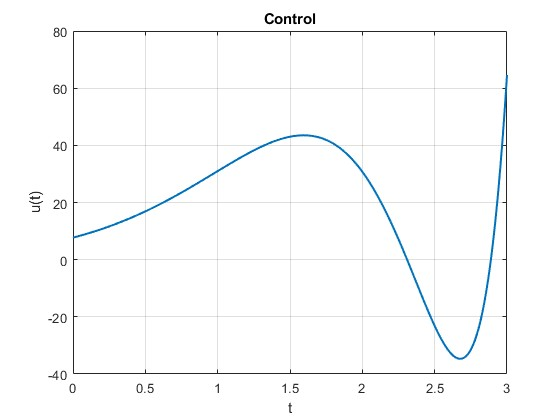
\includegraphics[width=\linewidth]{task_1_u_t.jpg}
            \caption{График $u(t)$}
            \label{fig:task_1_u_t}
        \end{subfigure}
        \hfill
        \begin{subfigure}{0.45\textwidth}
            \centering
            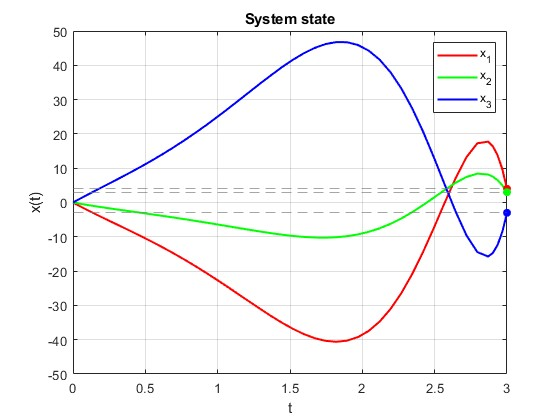
\includegraphics[width=\linewidth]{task_1_x_t.jpg}
            \caption{График $x(t)$}
            \label{fig:task_1_x_t}
        \end{subfigure}
        \caption{Графики для первого задания}
        \label{fig:task_1_modeling}
    \end{figure}
    \noindent Серыми пунктирными линиями на графике $x(t)$ отмечены координаты точки $x_1=\left[4\ 3\ -3\right]^T$.
    Как видим, система достигает состояния $x_1$ в момент времени $t_1=3$ -- $x_i$ сходятся к соответствующим пунктирным линиям.


    \subsection{Выводы}
    Все собственные числа матрицы $A$ управляемы, система полностью управляема. Моделирование системы подтвердило наши рассуждения.


    \section{Задание 2. Еще одно исследование управляемости}
    Рассмотрим систему
    $$
    \dot{x}=Ax+Bu,\text{ где }A=\begin{bmatrix}
        1 &-2 &3\\
        2 &-3 &2\\
        -2 &1 &-4
    \end{bmatrix},\ B=\begin{bmatrix}
        3\\
        1\\
        -1
    \end{bmatrix},\ x_1^{\prime}=\begin{bmatrix}
        4\\
        3\\
        -3
    \end{bmatrix},\ x_1^{\prime\prime}=\begin{bmatrix}
        3\\
        3\\
        -2
    \end{bmatrix}
    $$


    \subsection{Проверка точек на принадлежность управляемому подпространству}
    Чтобы проверить, принадлежит ли точка управляемому подпространству системы, необходимо найти матрицу управляемости
    и вычислить ее ранг. После этого создать расширенную матрицу -- матрица управляемости с точкой, которую проверяем на принадлежность
    управляемому подпространству системы. Смысл в том, что, если ранг расширенной матрицы будет равен рангу обычной матрицы управляемости,
    то данная точка уже существует в базисе, в котором задана система, а значит можно перевести систему в эту точку некоторым управлением из
    начальной точки (линейная зависимость). Если ранг больше, то точка выходит за пределы подпространства.


    Найдем матрицу управления $U$ и ее ранг. Ожидаем ранг, равный двум. Опустим вычисления, так как они аналогичны первому заданию. Программа для
    вычислений и построения графиков представлена на листинге \ref{task2} в приложении 2. Получаем
    $$
    U=\begin{bmatrix}
        B &AB &A^2B
    \end{bmatrix}=\begin{bmatrix}
    3    &-2    &-7\\
     1     &1    &-9\\
    -1    &-1     &9
    \end{bmatrix},\ \text{rank}\left[U\right]=2
    $$
    Создадим расширенные матрицы и вычислим их ранги
    $$
    U_{x_1^{\prime}}=\begin{bmatrix}
        U &x_1^{\prime}
    \end{bmatrix}=\begin{bmatrix}
    3    &-2    &-7     &4\\
     1     &1    &-9     &3\\
    -1    &-1     &9    &-3
    \end{bmatrix},\ \text{rank}\left[U_{x_1^{\prime}}\right]=2
    $$
    $$
    U_{x_1^{\prime\prime}}=\begin{bmatrix}
        U &x_1^{\prime\prime}
    \end{bmatrix}=\begin{bmatrix}
    3    &-2    &-7     &3\\
     1     &1    &-9     &3\\
    -1    &-1     &9    &-2
    \end{bmatrix},\ \text{rank}\left[U_{x_1^{\prime\prime}}\right]=3
    $$
    Выходит, что точка $x_1^{\prime}$ принадлежит управляемому подпространству системы, а $x_1^{\prime\prime}$ -- нет.
    Принимаем целевой точкой $x_1$ точку $x_1^{\prime}$. Далее все шаги аналогичны первому заданию.


    \subsection{Матрица управляемости}
    Сделаем вывод об управляемости системы по матрице управляемости.
    Система одноканальная -- один вход и один выход -- $U$ квадратная. Проверим определитель
    $$\det{\left[U\right]}=0$$
    Так как определитель равен нулю, то система является не полностью управляемой.
    Об этом уже говорил ранг $U$, меньший порядка системы.


    \subsection{Собственные числа и матрицы Хаутуса}
    Матрица $A$ такая же, как в первом задании. Мы уже вычислили ее собственные числа
    \begin{align*}
        &\lambda_1=-2\\
        &\lambda_{2,3}=-2\pm i
    \end{align*}
    и выяснили, что они асимптотически устойчивые, но могут быть неуправляемыми.
    Матрицы Хаутуса изменятся -- они зависят от $B$. Построим их и вычислим их ранги
    $$
    \text{rank}\left[A-\lambda_1 I\ B\right]=\text{rank}\begin{bmatrix}
        3 &-2 &3 &3\\
        2 &-1 &2 &1\\
        -2 &1 &-2 &-1
    \end{bmatrix}=2
    $$
    $$
    \text{rank}\left[A-\lambda_{2,3} I\ B\right]=\text{rank}\begin{bmatrix}
        3\pm i &-2 &3 &3\\
        2 &-1\pm i &2 &1\\
        -2 &1 &-2\pm i &-1
    \end{bmatrix}=3
    $$
    Выходит, что $\lambda_{2,3}=-2\pm i$ являются управляемыми, так как ранги их матриц Хаутуса равны порядку системы.
    Собственное число $\lambda_1=-2$ неуправляемое (ранг матрицы Хаутуса меньше порядка системы), но устойчивое -- система не полностью управляема, но стабилизируема.


    \subsection{Жорданова форма системы}
    Жорданово разложение матрицы $A$ не изменится, но изменится матрица входных воздействий, так как $B$ другая.
    Имеем
    $$
    A=P_{re}J_{re}P_{re}^{-1}=\begin{bmatrix}
        -1 &0.5 &-1.5\\
        0 &0 &-1\\
        1 &0 &1
    \end{bmatrix}\begin{bmatrix}
        -2 &0 &0\\
        0 &-2 &1\\
        0 &-1 &-2
    \end{bmatrix}\begin{bmatrix}
        0 &1 &1\\
        2 &-1 &2\\
        0 &-1 &0
    \end{bmatrix}
    $$
    Пересчитаем $B_{Jre}$
    $$
    B_{Jre}=P_{re}^{-1}B=\begin{bmatrix}
        0 &1 &1\\
        2 &-1 &2\\
        0 &-1 &0
    \end{bmatrix}\begin{bmatrix}
        3\\
        1\\
        -1
    \end{bmatrix}=\begin{bmatrix}
        0\\
        3\\
        -1
    \end{bmatrix}
    $$
    Таким образом, исследуем
    $$
    J_{re}\begin{bmatrix}
        -2 &0 &0\\
        0 &-2 &1\\
        0 &-1 &-2
    \end{bmatrix},\ B_{Jre}=\begin{bmatrix}
        0\\
        3\\
        -1
    \end{bmatrix}
    $$
    Все жордановы клетки относятся к различным собственным числам. Собственное число $\lambda_1=-2$ неуправляемое,
    а $\lambda_{2,3}=-2\pm i$ управляемые. Достаточное условие полной управляемости не выполнено -- первый элемент
    матрицы входных воздействий $B_{Jre}$ равен нулю -- система не полностью управляема.


    \subsection{Грамиан управляемости системы}
    Найдем Грамиан управляемости системы относительно времени $t_1=3$ аналогично первому заданию
    $$
    P\left(t_1=3\right)=\begin{bmatrix}
    3.625    &1.625   &-1.625\\
    1.625    &0.750   &-0.750\\
   -1.625   &-0.750    &0.750
    \end{bmatrix}
    $$
    Теперь найдем собственные числа Грамиана
    \begin{align*}
        \lambda_1=5.0943\\
        \lambda_2=0.0307\\
        \lambda_3=0.0000
    \end{align*}
    Так как одно из собственных чисел Грамиана равно нулю, то его определитель равен нулю, то есть Грамиан вырожденный.
    Это следует уже из неполного ранга матрицы управляемости. Система не полностью управляема -- в некотором направлении
    управлять системой не получится. В других же направлениях (двумерном подпространстве) система управляема.


    \subsection{Управление системой за определенное время}
    Найдем приближенное управление, переводящее систему из $x(0)=0$ в $x(t_1)=x_1$ за время $t_1$.
    Теперь в формуле необходимо использовать псевдообратную матрицу Грамиана, так как вследствие
    вырожденности обратную найти не получится
    $$u(t)=B^Te^{A^T(t_1-t)}\left[P(t_1)\right]^{+}x_1$$
    Подставим матрицы и $t_1$ в выражение
    $$
    u(t)=\begin{bmatrix}
        3\\
        1\\
        -1
    \end{bmatrix}^T
    e^{\begin{bmatrix}
        1 &-2 &3\\
        2 &-3 &2\\
        -2 &1 &-4
    \end{bmatrix}^T\left(3-t\right)}\begin{bmatrix}
        3.625    &1.625   &-1.625\\
        1.625    &0.750   &-0.750\\
       -1.625   &-0.750    &0.750
        \end{bmatrix}^{+}\begin{bmatrix}
            4\\
            3\\
            -3
        \end{bmatrix}
    $$
    После всех вычислений получим
    $$
    u(t)=\dfrac{-80001\cos{(3-t)}+360002\sin{(3-t)}}{5000e^4}  
    $$
    Аналогично первому заданию промоделируем систему. Результаты представлены на рис. \ref{fig:task_2_modeling}
    \begin{figure}[H]
        \centering
        \begin{subfigure}{0.45\textwidth}
            \centering
            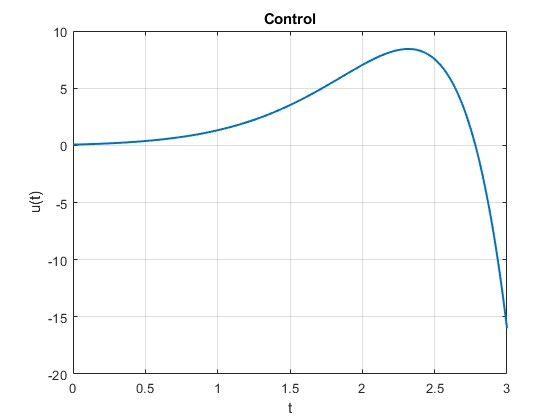
\includegraphics[width=\linewidth]{task_2_u_t.jpg}
            \caption{График $u(t)$}
            \label{fig:task_2_u_t}
        \end{subfigure}
        \hfill
        \begin{subfigure}{0.45\textwidth}
            \centering
            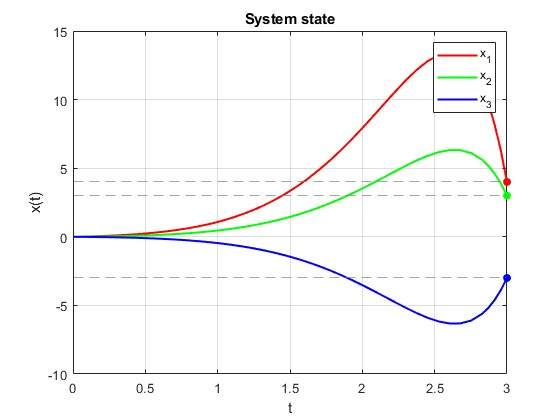
\includegraphics[width=\linewidth]{task_2_x_t.jpg}
            \caption{График $x(t)$}
            \label{fig:task_2_x_t}
        \end{subfigure}
        \caption{Графики для второго задания}
        \label{fig:task_2_modeling}
    \end{figure}
    \noindent Серыми пунктирными линиями на графике $x(t)$ отмечены координаты точки $x_1=\left[4\ 3\ -3\right]^T$.
    Как видим, система достигает состояния $x_1$ в момент времени $t_1=3$ -- $x_i$ сходятся к соответствующим пунктирным линиям.
    Это подтверждает, что точка $x_1^{\prime}$ принадлежит управляемому подпространству системы -- мы ее достигли, несмотря на не полную управляемость системы.


    \subsection{Выводы}
    Система не полностью управляема, но стабилизируема. Мы смогли найти приближенное управление для перевода системы из начального условия
    в точку $x_1$, принадлежащую управляемому подпространству системы, за конечное время $t_1$ и, продемонстрировали это, промоделировав систему.


    \section{Задание 3. Исследование наблюдаемости}
    Рассмотрим систему
    $$
    \begin{cases}
        \dot{x}=Ax,\\
        y=Cx,
    \end{cases} A=\begin{bmatrix}
        -16 &-27 &7\\
        6 &9 &-4\\
        -5 &-11 &0
    \end{bmatrix},\ C=\begin{bmatrix}
        2 &7 &1
    \end{bmatrix},
    $$
    $$f(t)=-9e^{-4t}\cos{(t)}+9e^{-4t}\sin{(t)}$$


    \subsection{Матрица наблюдаемости}
    Составим матрицу наблюдаемости системы и определим ее ранг. Порядок системы равен трем
    $$
    V=\begin{bmatrix}
        C\\
        CA\\
        CA^2
    \end{bmatrix}
    $$
    Найдем неизвестные
    $$
    CA=\begin{bmatrix}
        2 &7 &1
    \end{bmatrix}\begin{bmatrix}
        -16 &-27 &7\\
        6 &9 &-4\\
        -5 &-11 &0
    \end{bmatrix}=\begin{bmatrix}
    5 &-2 &-14
    \end{bmatrix}
    $$
    $$
    CA^2=\begin{bmatrix}
        2 &7 &1
    \end{bmatrix}\begin{bmatrix}
        -16 &-27 &7\\
        6 &9 &-4\\
        -5 &-11 &0
    \end{bmatrix}^2=\begin{bmatrix}
        2 &7 &1
    \end{bmatrix}
    \begin{bmatrix}
    59   &112    &-4\\
   -22   &-37     &6\\
    14    &36     &9
    \end{bmatrix}=\begin{bmatrix}
        -22     &1    &43
    \end{bmatrix}
    $$
    Таким образом, получаем матрицу наблюдаемости
    $$
    V=\begin{bmatrix}
    2     &7     &1\\
    5    &-2   &-14\\
   -22     &1    &43
    \end{bmatrix}
    $$
    Определим ее ранг
    $$
    \text{rank}\left[V\right]=\text{rank}\begin{bmatrix}
        2     &7     &1\\
        5    &-2   &-14\\
       -22     &1    &43
    \end{bmatrix}=3
    $$
    Ранг матрицы наблюдаемости равен порядку системы $n=3$, следовательно, система полностью наблюдаема.
    Так как выход один и матрица $V$ квадратная, достаточно было сравнить ее определитель с нулем.


    \subsection{Собственные числа и матрицы Хаутуса}
    Собственные числа находим аналогично первому заданию. Предоставим вычисления \texttt{MATLAB}. Программа
    находится на листинге \ref{task3} в приложении 3
    $$
    \det{\left[\lambda I-A\right]}=0
    $$
    Получаем
    \begin{align*}
    &\lambda_1=1\\
    &\lambda_{2,3}=-4\pm i
    \end{align*}
    Видим, что $\lambda_1>0$ -- неустойчивое, нужна наблюдаемость. Действительная часть
    $\lambda_{2,3}$ меньше нуля, следовательно, они асимптотически устойчивые, но могут быть ненаблюдаемыми.
    Для проверки найдем матрицы Хаутуса для наблюдаемости
    $$
    \mathcal{H}=\begin{bmatrix}
        A-\lambda I\\
        C
    \end{bmatrix}
    $$
    Если ранг этой матрицы для конкретного $\lambda_i$ равен порядку системы $n$, то это собственное число наблюдаемо.
    Определим матрицы и их ранги
    $$
    \text{rank}\begin{bmatrix}
        A-\lambda_1 I\\
        C
    \end{bmatrix}=\text{rank}\begin{bmatrix}
    -17  &-27    &7\\
    6    &8   &-4\\
   -5  &-11   &-1\\
    2    &7    &1
    \end{bmatrix}=3
    $$
    $$
    \text{rank}\begin{bmatrix}
        A-\lambda_{2,3} I\\
        C
    \end{bmatrix}=\text{rank}\begin{bmatrix}
    -12\pm i &-27   &7\\
    6  &13\pm i  &-4\\
    -5 &-11   &4\pm i\\
    2   &7   &1
    \end{bmatrix}=3
    $$
    Ранги матриц Хаутуса для каждого собственного числа матрицы $A$ равны порядку
    системы, следовательно, все собственные числа являются наблюдаемыми. Из этого
    же следует, что система полностью наблюдаема.


    \subsection{Жорданова форма системы}
    Найдем жорданово разложение матрицы в \texttt{MATLAB} и приведем к вещественному виду
    $$
    A=PJP^{-1}=\begin{bmatrix} 
    2	&3-2i	&3+2i\\
    -1	&-1+i	&-1-i\\
    1	   &1	   &1 
    \end{bmatrix}\begin{bmatrix}
    1	   &0	   &0\\
    0	&-4-i	   &0\\
    0	   &0	&-4+i
    \end{bmatrix}\begin{bmatrix}
    -1	     &-2	   &1\\
    0.5	&1-0.5i	&-0.5i\\
    0.5	&1+0.5i	 &0.5i
    \end{bmatrix}
    $$
    $$
    A=P_{re}J_{re}P_{re}^{-1}=\begin{bmatrix}
    2    &-2     &3\\
    -1     &1    &-1\\
     1     &0     &1
    \end{bmatrix}\begin{bmatrix}
    1     &0     &0\\
    0    &-4     &1\\
    0    &-1    &-4
    \end{bmatrix}\begin{bmatrix}
    -1    &-2     &1\\
    0     &1     &1\\
    1     &2     &0
    \end{bmatrix}
    $$
    Найдем матрицу выходов $C_{Jre}$ в базисе собственных векторов матрицы $A$
    $$
    C_{Jre}=CP_{re}=\begin{bmatrix}
        2 &7 &1
    \end{bmatrix}\begin{bmatrix}
        2    &-2     &3\\
        -1     &1    &-1\\
         1     &0     &1
    \end{bmatrix}=\begin{bmatrix}
        -2     &3     &0
    \end{bmatrix}
    $$
    Итого имеем
    $$J_{re}=\begin{bmatrix}
        1     &0     &0\\
        0    &-4     &1\\
        0    &-1    &-4
    \end{bmatrix},\ C_{Jre}=\begin{bmatrix}
        -2     &3     &0
    \end{bmatrix}
    $$
    Все жордановы клетки относятся к различным собственным числам. Видим, что $\lambda_{1},\lambda_{2}$ наблюдаемы, а
    $\lambda_3$ -- нет (см. элементы соответствующих столбцов $C_{Jre}$). Из наблюдаемости $\lambda_1,\lambda_2,\lambda_3$ нельзя сделать вывод, что система полностью наблюдаема. Достаточное условие полной наблюдаемости системы
    в нашем случае -- не равенство нулю первого и [второго или третьего] элементов столбцов матрицы выходов $C_{Jre}$. Так как
    оно выполняется, то система является полностью наблюдаемой.


    \subsection{Грамиан наблюдаемости системы}
    Найдем Грамиан наблюдаемости системы относительно времени $t_1=3$
    $$Q(t_1)=\int\limits_{0}^{t_1}e^{A^Tt}C^TCe^{At}\,dt$$
    Предоставим вычисления \texttt{MATLAB}. Получим следующий результат
    $$
    Q(t_1=3)=10^3\times\begin{bmatrix}
    0.8061    &1.6141   &-0.8035\\
    1.6141    &3.2332   &-1.6078\\
   -0.8035   &-1.6078    &0.8023
    \end{bmatrix}
    $$
    Найдем собственные числа Грамиана наблюдаемости
    \begin{align*}
    &\lambda_1=4.8393\cdot 10^3\\
    &\lambda_2=0.0000\cdot 10^3\\
    &\lambda_3=0.0023\cdot 10^3
    \end{align*}
    У Грамиана наблюдаемости присутствует нулевое собственное число -- он вырожденный, система не полностью наблюдаема.
    При этом другие собственные числа достаточно велики -- в некоторых неправлениях система хорошо наблюдаема. Такой результат
    может говорить о том, что на практике какое-то состояние системы не получится восстановить за конечное время $t_1$. При
    этом теоретически система полностью наблюдаема.


    \subsection{Определение начальных условий системы}
    Пусть выход системы $y(t)$ подчиняется закону $y(t)=f(t)$ на временном интервале $t\in\left[0,t_1\right]$.
    Определим начальные условия системы по формуле
    $$
    x(0)=\left[Q(t_1)\right]^+\int\limits_{0}^{t_1}e^{A^Tt}C^Ty(t)\,dt
    $$
    Вместо обратной матрицы Грамиана используем псевдообратную (определитель равен нулю).
    Подставим матрицы, $t_1$ и $y(t)$
    $$
    x(0)=\begin{bmatrix}
        806.1	&1614.1	&-803.5\\
        1614.1	 &3233.2	&-1607.8\\
        -803.5	 &-1607.8	&802.3 
    \end{bmatrix}^+9\int\limits_{0}^{3}e^{\begin{bmatrix}
        -16 &-27 &7\\
        6 &9 &-4\\
        -5 &-11 &0
    \end{bmatrix}^Tt-4t}\begin{bmatrix}
        2\\ 7\\ 1
    \end{bmatrix}\left(\sin{(t)}-\cos{(t)}\right)
    $$
    Предоставим вычисления \texttt{MATLAB}. Получаем следующий результат
    $$
    x(0)=\begin{bmatrix}
    15\\
   -6\\
    3
    \end{bmatrix}
    $$
    Получили начальные условия системы, соответсвующие выходу $y(t)=f(t)$. Выполним моделирование системы аналогично первому заданию.
    Программа для построения графиков находится в приложении 3. Графики представлены на рисунке \ref{fig:task_3_modeling}
    \begin{figure}[H]
        \centering
        \begin{subfigure}{0.45\textwidth}
            \centering
            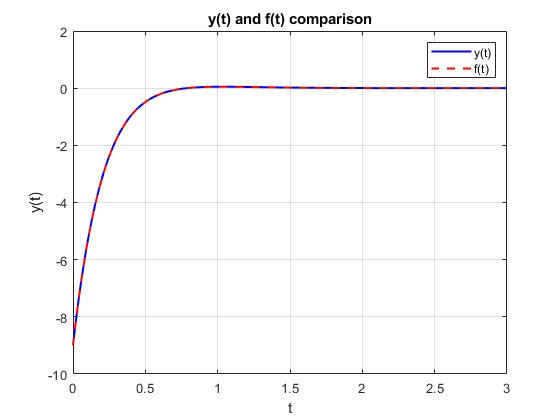
\includegraphics[width=\linewidth]{task_3_y_t_f_t.jpg}
            \caption{График $y(t)$ и $f(t)$}
            \label{fig:task_3_y_t_f_t}
        \end{subfigure}
        \hfill
        \begin{subfigure}{0.45\textwidth}
            \centering
            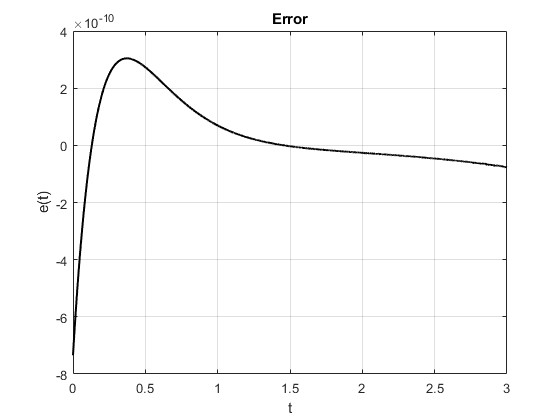
\includegraphics[width=\linewidth]{task_3_err.jpg}
            \caption{График $e(t)=y(t)-f(t)$}
            \label{fig:task_3_err}
        \end{subfigure}
        \caption{Графики для третьего задания}
        \label{fig:task_3_modeling}
    \end{figure}
    \noindent Графики $y(t)$ и $f(t)$ почти совпадают. На графике ошибки видим очень маленькие значения ($\times10^{-10}$).
    Логично, что наибольшая ошибка будет в момент наибольшего изменения состояния системы, а дальше будет уменьшаться, что видим на рис. \ref{fig:task_3_err},
    сопоставляя $t$ с рис. \ref{fig:task_3_y_t_f_t}.


    \subsection{Выводы}
    Теоретически система полностью наблюдаема (критерий Калмана, матрицы Хаутуса, жорданова форма системы), но практически есть направления, в которых система ненаблюдаема (Грамиан наблюдаемости).
    Начальные условия при заданной $f(t)$ были найдены, система была успешно промоделирована.


    \section{Задание 4. Еще одно исследование наблюдаемости}
    Рассмотрим систему
    $$
    \begin{cases}
        \dot{x}=Ax,\\
        y=Cx,
    \end{cases} A=\begin{bmatrix}
        -16 &-27 &7\\
        6 &9 &-4\\
        -5 &-11 &0
    \end{bmatrix},\ C=\begin{bmatrix}
        0 &-5 &-5
    \end{bmatrix},
    $$
    $$f(t)=-9e^{-4t}\cos{(t)}+9e^{-4t}\sin{(t)}$$


    \subsection{Матрица наблюдаемости}
    Составим аналогично предыдущему заданию матрицу наблюдаемости и определим ее ранг
    (порядок системы $n=3$, программа представлена на листинге \ref{task4} в приложении 4)
    $$
    V=\begin{bmatrix}
        C\\
        CA\\
        CA^2
    \end{bmatrix},\ CA=\begin{bmatrix}
        -5\\    10\\    20
    \end{bmatrix}^T,\ CA^2=\begin{bmatrix}
        40\\     5\\   -75
    \end{bmatrix}^T
    $$
    Получаем
    $$
    V=\begin{bmatrix}
    0    &-5    &-5\\
    -5    &10    &20\\
    40     &5   &-75
    \end{bmatrix},\ \text{rank}\left[V\right]=2,\ \det{\left[V\right]}=0
    $$
    Ранг матрицы наблюдаемости меньше порядка системы, определитель равен нулю, система не полностью наблюдаема.
    Существуют ненаблюдаемые состояния, которые не влияют на $y(t)$.


    \subsection{Собственные числа и матрицы Хаутуса}
    Матрица $A$ такая же, как в задании №3 -- собственные числа не изменятся. Имеем
    \begin{align*}
        &\lambda_1=1\\
        &\lambda_{2,3}=-4\pm i
    \end{align*}
    Выводы по собственным числам аналогичны предыдущему заданию. Построим матрицы Хаутуса
    $$
    \mathcal{H}=\begin{bmatrix}
        A-\lambda I\\
        C
    \end{bmatrix}
    $$
    Вычисления производятся в \texttt{MATLAB}. Определим эти матрицы и их ранги
    $$
    \text{rank}\begin{bmatrix}
        A-\lambda_1 I\\
        C
    \end{bmatrix}=\text{rank}\begin{bmatrix}
    -17  &-27    &7\\
    6    &8   &-4\\
   -5  &-11   &-1\\
    0   &-5   &-5
    \end{bmatrix}=2
    $$
    $$
    \text{rank}\begin{bmatrix}
        A-\lambda_{2,3} I\\
        C
    \end{bmatrix}=\text{rank}\begin{bmatrix}
        -12\pm i  &-27    &7\\
        6    &13\pm i   &-4\\
       -5  &-11   &4\pm i\\
        0   &-5   &-5
    \end{bmatrix}=3
    $$
    Видим, что ранг матрицы Хаутуса для $\lambda_1$ меньше порядка системы -- собственное число $\lambda_1$ ненаблюдаемое.
    Собственные числа $\lambda_{2,3}$ наблюдаемы, ранги их матриц Хаутуса совпадают с порядком системы. Таким образом, система не полностью наблюдаема.


    \subsection{Жорданова форма системы}
    Жорданова форма системы будет такая же, как в задании №3
    $$
    A=P_{re}J_{re}P_{re}^{-1}=\begin{bmatrix}
        2    &-2     &3\\
        -1     &1    &-1\\
         1     &0     &1
        \end{bmatrix}\begin{bmatrix}
        1     &0     &0\\
        0    &-4     &1\\
        0    &-1    &-4
        \end{bmatrix}\begin{bmatrix}
        -1    &-2     &1\\
        0     &1     &1\\
        1     &2     &0
        \end{bmatrix}
    $$
    Найдем матрицу выходов $C_{Jre}$ в базисе собственных векторов матрицы $A$
    $$C_{Jre}=CP_{re}=\begin{bmatrix}
        0 &-5 &-5
    \end{bmatrix}\begin{bmatrix}
        2    &-2     &3\\
        -1     &1    &-1\\
         1     &0     &1
    \end{bmatrix}=\begin{bmatrix}
    0	&-5	&0
    \end{bmatrix}$$
    Итого имеем
    $$
    J_{re}=\begin{bmatrix}
        1     &0     &0\\
        0    &-4     &1\\
        0    &-1    &-4
    \end{bmatrix},\ C_{Jre}=\begin{bmatrix}
        0	&-5	&0
    \end{bmatrix}
    $$
    Все жордановы клетки относятся к различным собственным числам. Видим, что наблюдаемым является
    только собственное число $\lambda_2$, так как элемент соответствующего столбца матрицы выходов не равен нулю.
    Остальные собственные числа ненаблюдаемы. Достаточное условие полной наблюдаемости системы не выполнено --
    первый элемент матрицы выходов равен нулю. Следовательно, система не полностью наблюдаема.


    \subsection{Грамиан наблюдаемости системы}
    Вычислим Грамиан наблюдаемости системы относительно времени $t_1=3$ аналогично заданию №3
    $$
    Q(t_1=3)=\begin{bmatrix}
    0.0919    &0.5515    &0.3676\\
    0.5515    &4.8713    &3.7684\\
    0.3676    &3.7684    &3.0331
    \end{bmatrix}
    $$
    Найдем собственные числа Грамиана наблюдаемости
    \begin{align*}
    &\lambda_1=7.8871\\
    &\lambda_2=-0.0000\\
    &\lambda_3=0.1093
    \end{align*}
    Видим, что у Грамиана наблюдаемости $\lambda_2=0$. Следовательно, Грамиан вырожденный.
    Другие же собственные числа наблюдаемы. Вывод -- система не полностью наблюдаема.
    

    \subsection{Определение начальных условий системы}
    Определим начальные условия системы аналогично заданию №3
    $$
    x(0)=\begin{bmatrix}
        0.0919    &0.5515    &0.3676\\
        0.5515    &4.8713    &3.7684\\
        0.3676    &3.7684    &3.0331
    \end{bmatrix}^+9\int\limits_{0}^{3}e^{\begin{bmatrix}
        -16 &-27 &7\\
        6 &9 &-4\\
        -5 &-11 &0
    \end{bmatrix}^Tt-4t}\begin{bmatrix}
        0\\
        -5\\
        -5
    \end{bmatrix}\left(\sin{(t)}-\cos{(t)}\right)
    $$
    Проведя вычисления в \texttt{MATLAB}, получаем
    $$
    x(0)=\begin{bmatrix}
    -1.2\\
   -0.3\\
    2.1
    \end{bmatrix}
    $$
    Получили начальные условия системы, соответсвующие выходу $y(t)=f(t)$.
    Выполним моделирование системы аналогично третьему заданию. 
    Программа для построения графиков находится в приложении 4.
    Графики представлены на рисунке \ref{fig:task_4_modeling}
    \begin{figure}[H]
        \centering
        \begin{subfigure}{0.45\textwidth}
            \centering
            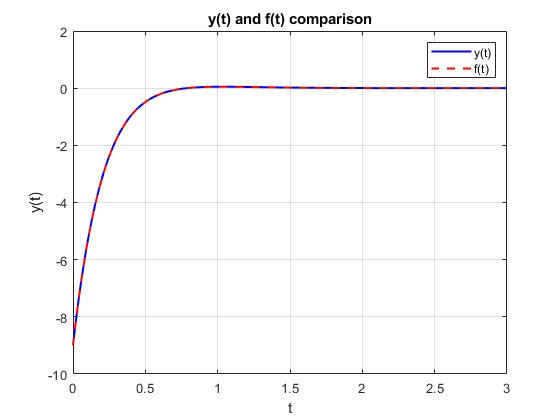
\includegraphics[width=\linewidth]{task_4_y_t_f_t.jpg}
            \caption{График $y(t)$ и $f(t)$}
            \label{fig:task_4_y_t_f_t}
        \end{subfigure}
        \hfill
        \begin{subfigure}{0.45\textwidth}
            \centering
            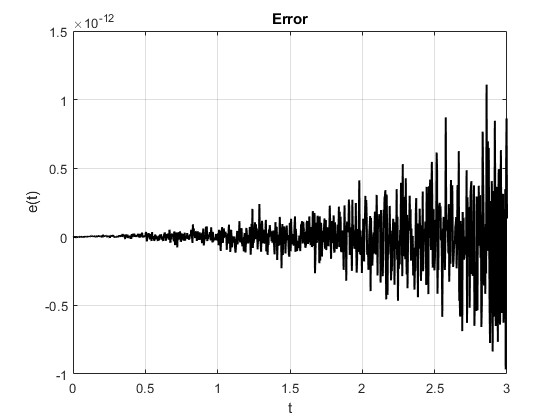
\includegraphics[width=\linewidth]{task_4_err.jpg}
            \caption{График $e(t)=y(t)-f(t)$}
            \label{fig:task_4_err}
        \end{subfigure}
        \caption{Графики для четвертого задания}
        \label{fig:task_4_modeling}
    \end{figure}
    \noindent График $y(t)$ почти совпадает с $f(t)$. Несмотря на то, что ошибка очень мала ($\times10^{-12}$),
    при увеличении $t$ (приближении к $t_1$) она хаотически возрастает по модулю. Либо это погрешности численного решения,
    либо особенности системы.


    \subsection{Другие начальные условия}
    ...


    \subsection{Вывод}
    ...


    \section{Приложения}
    \subsection{Приложение 1}
    \begin{lstlisting}[label=task1, caption={Программа для первого задания}]
    % input data
    A = [1 -2 3; 2 -3 2; -2 1 -4];
    B = [-3; -1; 3];
    x1 = [4; 3; -3];
    t1 = 3;

    % controllability matrix
    U = [B A*B A*A*B];
    r = rank(U);
    disp(U);
    disp(r);

    % A matrix eigenvalues
    A_e = eig(A);
    disp(A_e);

    % Houtus matrices
    H_1 = [A-A_e(1)*eye(3) B];
    r_1 = rank(H_1);
    disp(H_1);
    disp(r_1);

    H_2 = [A-A_e(2)*eye(3) B];
    r_2 = rank(H_2);
    disp(H_2);
    disp(r_2);

    H_3 = [A-A_e(3)*eye(3) B];
    r_3 = rank(H_3);
    disp(H_3);
    disp(r_3);

    % Jordan matrix
    [P, J] = jordan(A);
    P1(:,1) = real(P(:,1));
    P1(:,2) = imag(P(:,2));
    P1(:,3) = real(P(:,3));
    P1_inv = P1^-1; 
    J_re = P1_inv * A * P1;
    B_jre = P1_inv * B;
    disp(P1);
    disp(P1_inv);
    disp(J_re);
    disp(B_jre);

    % gramian
    integrand = @(t) expm(A * t) * (B * B') * expm(A' * t);
    P_t1 = integral(@(t) integrand(t), 0, t1, 'ArrayValued', true);
    disp(P_t1);

    % gramian eigenvalues
    e = eig(P_t1);
    disp(e);

    % u_t
    u_t = @(t) B' * expm(A' * (t1 - t)) * inv(P_t1) * x1;

    % u_t modeling
    time = linspace(0, t1, 1000);

    control = arrayfun(@(t) u_t(t), time, 'UniformOutput', false);
    control = cell2mat(control);

    figure;
    plot(time, control, 'LineWidth', 1.5);
    xlabel('t');
    ylabel('u(t)');
    title('Control');
    grid on;

    % x_t
    dxdt = @(t, x) A * x + B * u_t(t);

    % x_t modeling
    [t, x] = ode45(dxdt, [0 t1], [0; 0; 0]);

    figure;
    plot(t, x, 'LineWidth', 1.5);
    yline(x1(1), '--', 'Color', [0.5 0.5 0.5]); % x_1
    yline(x1(2), '--', 'Color', [0.5 0.5 0.5]); % x_2
    yline(x1(3), '--', 'Color', [0.5 0.5 0.5]); % x_3
    xlabel('t');
    ylabel('x(t)');
    legend('x_1', 'x_2', 'x_3');
    title('System state');
    grid on;
    \end{lstlisting}


    \subsection{Приложение 2}
    \begin{lstlisting}[label=task2, caption={Программа для второго задания}]
    % input data
    A = [1 -2 3; 2 -3 2; -2 1 -4];
    B = [3; 1; -1];
    x1p = [4; 3; -3];
    x1pp = [3; 3; -2];
    t1 = 3;

    % controllability matrix
    U = [B A*B A*A*B];
    r = rank(U);
    detU = det(U);
    disp(U);
    disp(r);
    disp(detU)

    % check x1p in subspace
    U_x1p = [U x1p];
    r_x1p = rank(U_x1p);
    disp(U_x1p);
    disp(r_x1p);

    % check x1pp in subspace
    U_x1pp = [U x1pp];
    r_x1pp = rank(U_x1pp);
    disp(U_x1pp);
    disp(r_x1pp);

    if r_x1p == r
        x1 = x1p;
    else
        x1 = x1pp;
    end
    disp(x1)

    % A matrix eigenvalues
    A_e = eig(A);
    disp(A_e);

    % Houtus matrices
    H_1 = [A-A_e(1)*eye(3) B];
    r_1 = rank(H_1);
    disp(H_1);
    disp(r_1);

    H_2 = [A-A_e(2)*eye(3) B];
    r_2 = rank(H_2);
    disp(H_2);
    disp(r_2);

    H_3 = [A-A_e(3)*eye(3) B];
    r_3 = rank(H_3);
    disp(H_3);
    disp(r_3);

    % Jordan matrix
    [P, J] = jordan(A);
    P1(:,1) = real(P(:,1));
    P1(:,2) = imag(P(:,2));
    P1(:,3) = real(P(:,3));
    P1_inv = P1^-1; 
    J_re = P1_inv * A * P1;
    B_jre = P1_inv * B;
    disp(P1);
    disp(P1_inv);
    disp(J_re);
    disp(B_jre);

    % gramian
    integrand = @(t) expm(A * t) * (B * B') * expm(A' * t);
    P_t1 = integral(@(t) integrand(t), 0, t1, 'ArrayValued', true);
    disp(P_t1);

    % gramian eigenvalues
    e = eig(P_t1);
    disp(e);

    % u_t
    u_t = @(t) B' * expm(A' * (t1 - t)) * pinv(P_t1) * x1;
    disp(pinv(P_t1));

    % u_t modeling
    time = linspace(0, t1, 1000);

    control = arrayfun(@(t) u_t(t), time, 'UniformOutput', false);
    control = cell2mat(control);

    figure;
    plot(time, control, 'LineWidth', 1.5);
    xlabel('t');
    ylabel('u(t)');
    title('Control');
    grid on;

    % x_t
    dxdt = @(t, x) A * x + B * u_t(t);

    % x_t modeling
    [t, x] = ode45(dxdt, [0 t1], [0; 0; 0]);

    figure;
    plot(t, x, 'LineWidth', 1.5);
    yline(x1(1), '--', 'Color', [0.5 0.5 0.5]); % x_1
    yline(x1(2), '--', 'Color', [0.5 0.5 0.5]); % x_2
    yline(x1(3), '--', 'Color', [0.5 0.5 0.5]); % x_3
    xlabel('t');
    ylabel('x(t)');
    legend('x_1', 'x_2', 'x_3');
    title('System state');
    grid on;
    \end{lstlisting}


    \subsection{Приложение 3}
    \begin{lstlisting}[label=task3, caption={Программа для третьего задания}]
    % input data
    A = [-16 -27 7; 6 9 -4; -5 -11 0];
    C = [2 7 1];
    f_t = @(t) -9 * exp(-4 * t) * cos(t) + 9 * exp(-4 * t) * sin(t);
    t1 = 3;

    % observability matrix
    V = [C; C*A; C*A^2];
    r = rank(V);
    disp(A^2);
    disp(V);
    disp(r);

    % A matrix eigenvalues
    A_e = eig(A);
    disp(A_e);

    % Houtus matrices
    H_1 = [A-A_e(1)*eye(3); C];
    r_1 = rank(H_1);
    disp(H_1);
    disp(r_1);

    H_2 = [A-A_e(2)*eye(3); C];
    r_2 = rank(H_2);
    disp(H_2);
    disp(r_2);

    H_3 = [A-A_e(3)*eye(3); C];
    r_3 = rank(H_3);
    disp(H_3);
    disp(r_3);

    % Jordan matrix
    [P, J] = jordan(A);
    P1(:,1) = real(P(:,1));
    P1(:,2) = imag(P(:,2));
    P1(:,3) = real(P(:,3));
    P1_inv = P1^-1; 
    J_re = P1_inv * A * P1;
    C_jre = C * P1;
    disp(P1);
    disp(P1_inv);
    disp(J_re);
    disp(C_jre);

    % gramian
    integrand = @(t) expm(A' * t) * (C' * C) * expm(A * t);
    Q_t1 = integral(@(t) integrand(t), 0, t1, 'ArrayValued', true);
    disp(Q_t1);

    % gramian eigenvalues
    e = eig(Q_t1);
    disp(e);

    % initial conditions x(0)
    integrand_x0 = @(t) expm(A' * t) * C' * f_t(t);
    X_int = integral(@(t) integrand_x0(t), 0, t1, 'ArrayValued', true);
    Q_t1_pinv = pinv(Q_t1);
    x0 = Q_t1_pinv * X_int;
    disp(Q_t1_pinv);
    disp(x0);

    % system modeling
    x_t = @(t) expm(A * t) * x0; 
    y_t = @(t) C * x_t(t);

    time = linspace(0, t1, 1000);
    y_arr = arrayfun(y_t, time);
    f_arr = arrayfun(f_t, time);

    figure;
    plot(time, y_arr, 'b', 'LineWidth', 1.5); hold on;
    plot(time, f_arr, 'r--', 'LineWidth', 1.5);
    xlabel('t');
    ylabel('y(t)');
    legend('y(t)', 'f(t)');
    title('y(t) and f(t) comparison');
    grid on;

    err = y_arr - f_arr;

    figure;
    plot(time, err, 'k', 'LineWidth', 1.5);
    xlabel('t');
    ylabel('e(t)');
    title('Error');
    grid on;
    \end{lstlisting}


    \subsection{Приложение 4}
    \begin{lstlisting}[label=task4, caption={Программа для четвертого задания}]
        to be done
    \end{lstlisting}
\end{document}